
\chapter[Lý thuyết: Động cơ không đồng bộ ba pha]{Lý thuyết: Động cơ không đồng bộ ba pha}
\section{Lý thuyết}
\subsection {Định nghĩa}
Động cơ điện xoay chiều (động cơ không đồng bộ ba pha) là thiết bị biến đổi điện năng thành cơ năng dựa trên hiện tượng cảm ứng điện từ và tác dụng của từ trường quay.
\subsection{Cấu tạo}
\begin{itemize}
	\item Stato: là bộ phận tạo nên từ trường quay gồm 3 cuộn dây giống nhau, đặt lệch nhau $120^ {\circ}$.
	\item Rôto: là khung dây dẫn có thể quay dưới tác dụng của từ trường quay. Để tăng thêm hiệu quả, người ta ghép nhiều khung dây dẫn giống nhau có trục quay chung tạo thành một cái lồng hình trụ, mặt bên tạo bởi nhiều thanh kim loại song song (rôto lồng sóc).
\end{itemize}
\begin{center}
	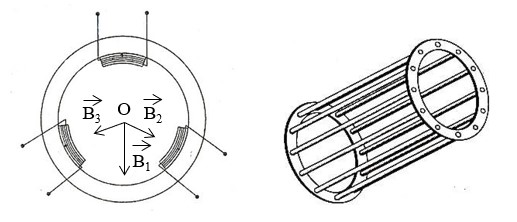
\includegraphics[scale=1.0]{VN12-PH-23-L-016-1-V2-01.jpg}
\end{center}
\subsection {Nguyên tắc hoạt động}
\begin{itemize}
	\item Tạo ra từ trường quay bằng cách cho dòng điện xoay chiều 3 pha đi vào trong stato gồm 3 cuộn dây giống nhau, đặt lệch nhau $120^\circ$ trên một giá tròn thì trong không gian giữa 3 cuộn dây sẽ có một từ trường quay với tần số góc bằng tần số góc $\omega$ của dòng điện xoay chiều.
	\item Đặt trong từ trường quay một rôto lồng sóc có thể quay xung quanh trục trùng với trục quay của từ trường.
	\item Rôto lồng sóc quay do tác dụng của từ trường quay với tốc độ nhỏ hơn tốc độ của từ trường. Chuyển động quay này được sử dụng để làm quay các máy khác.
\end{itemize}


\section{Mục tiêu bài học - Ví dụ minh họa}
\begin{dang}{Ghi nhớ cấu tạo và nguyên tắc hoạt động của động cơ không đồng bộ ba pha}
	\viduii{2}{Chọn phát biểu đúng.
		\begin{mcq}
			\item Chỉ có dòng điện ba pha mới tạo được từ trường quay.
			\item Rôto của động cơ không đồng bộ quay với tốc độ góc của từ trường quay.
			\item Từ trường quay trong động cơ không đồng bộ luôn thay đổi cả về hướng và trị số.
			\item Tốc độ góc của động cơ không đồng bộ phụ thuộc vào tốc độ quay của từ trường và momen cản.
		\end{mcq}
	}
	{	\begin{center}
			\textbf{Hướng dẫn giải}
		\end{center}
		
		\begin{itemize}
			\item Ngoài dòng điện ba pha có nhiều cách để tạo ra từ trường quay $\Rightarrow $ Câu A sai.
			\item Rôto của động cơ không đồng bộ ba pha quay với tốc độ góc nhỏ hơn tốc độ góc từ trường quay $\Rightarrow $ Câu B sai.
			\item Từ trường quay trong động cơ không đồng bộ 3 pha có trị số không đổi và luôn bằng $ 1,5B_0$ $\Rightarrow $ Câu C sai.
			\item Tốc độ góc của động cơ không đồng bộ phụ thuộc vào tốc độ quay của từ trường và momen cản $\Rightarrow$ Câu D đúng.
		\end{itemize}
		
		\textbf{Đáp án: D.}
	}
	\viduii{2}{Phát biểu nào sau đây về động cơ không đồng bộ ba pha là \textbf{sai}?
		\begin{mcq}
			\item Hai bộ phận chính của động cơ là rôto và stato.
			\item Bộ phận tạo ra từ trường quay là stato.
			\item Nguyên tắc hoạt động của động cơ chỉ dựa trên tương tác từ giữa nam châm và dòng điện.
			\item Có thể chế tạo động cơ không đồng bộ ba pha với công suất lớn.
		\end{mcq}
	}
	{	\begin{center}
			\textbf{Hướng dẫn giải}
		\end{center}
		
		Vì nguyên tắc hoạt động của động cơ không đồng bộ 3 pha: 
		
		Cho dòng điện 3 pha đi vào 3 cuộn dây giống hệt nhau đặt lệch nhau $120^\circ$ trên vành tròn của stato thì trên trục của stato có một từ trường quay. Nếu đặt một khung dây kín có trục quay trùng với trục của stato thì khung dây sẽ quay không đồng bộ theo từ trường quay này.
		
		\textbf{Đáp án: C.}
	}
\end{dang}
